% Options for packages loaded elsewhere
\PassOptionsToPackage{unicode}{hyperref}
\PassOptionsToPackage{hyphens}{url}
\PassOptionsToPackage{dvipsnames,svgnames,x11names}{xcolor}
%
\documentclass[
  letterpaper,
  DIV=11,
  numbers=noendperiod]{scrartcl}

\usepackage{amsmath,amssymb}
\usepackage{iftex}
\ifPDFTeX
  \usepackage[T1]{fontenc}
  \usepackage[utf8]{inputenc}
  \usepackage{textcomp} % provide euro and other symbols
\else % if luatex or xetex
  \usepackage{unicode-math}
  \defaultfontfeatures{Scale=MatchLowercase}
  \defaultfontfeatures[\rmfamily]{Ligatures=TeX,Scale=1}
\fi
\usepackage{lmodern}
\ifPDFTeX\else  
    % xetex/luatex font selection
\fi
% Use upquote if available, for straight quotes in verbatim environments
\IfFileExists{upquote.sty}{\usepackage{upquote}}{}
\IfFileExists{microtype.sty}{% use microtype if available
  \usepackage[]{microtype}
  \UseMicrotypeSet[protrusion]{basicmath} % disable protrusion for tt fonts
}{}
\makeatletter
\@ifundefined{KOMAClassName}{% if non-KOMA class
  \IfFileExists{parskip.sty}{%
    \usepackage{parskip}
  }{% else
    \setlength{\parindent}{0pt}
    \setlength{\parskip}{6pt plus 2pt minus 1pt}}
}{% if KOMA class
  \KOMAoptions{parskip=half}}
\makeatother
\usepackage{xcolor}
\setlength{\emergencystretch}{3em} % prevent overfull lines
\setcounter{secnumdepth}{-\maxdimen} % remove section numbering
% Make \paragraph and \subparagraph free-standing
\ifx\paragraph\undefined\else
  \let\oldparagraph\paragraph
  \renewcommand{\paragraph}[1]{\oldparagraph{#1}\mbox{}}
\fi
\ifx\subparagraph\undefined\else
  \let\oldsubparagraph\subparagraph
  \renewcommand{\subparagraph}[1]{\oldsubparagraph{#1}\mbox{}}
\fi

\usepackage{color}
\usepackage{fancyvrb}
\newcommand{\VerbBar}{|}
\newcommand{\VERB}{\Verb[commandchars=\\\{\}]}
\DefineVerbatimEnvironment{Highlighting}{Verbatim}{commandchars=\\\{\}}
% Add ',fontsize=\small' for more characters per line
\usepackage{framed}
\definecolor{shadecolor}{RGB}{241,243,245}
\newenvironment{Shaded}{\begin{snugshade}}{\end{snugshade}}
\newcommand{\AlertTok}[1]{\textcolor[rgb]{0.68,0.00,0.00}{#1}}
\newcommand{\AnnotationTok}[1]{\textcolor[rgb]{0.37,0.37,0.37}{#1}}
\newcommand{\AttributeTok}[1]{\textcolor[rgb]{0.40,0.45,0.13}{#1}}
\newcommand{\BaseNTok}[1]{\textcolor[rgb]{0.68,0.00,0.00}{#1}}
\newcommand{\BuiltInTok}[1]{\textcolor[rgb]{0.00,0.23,0.31}{#1}}
\newcommand{\CharTok}[1]{\textcolor[rgb]{0.13,0.47,0.30}{#1}}
\newcommand{\CommentTok}[1]{\textcolor[rgb]{0.37,0.37,0.37}{#1}}
\newcommand{\CommentVarTok}[1]{\textcolor[rgb]{0.37,0.37,0.37}{\textit{#1}}}
\newcommand{\ConstantTok}[1]{\textcolor[rgb]{0.56,0.35,0.01}{#1}}
\newcommand{\ControlFlowTok}[1]{\textcolor[rgb]{0.00,0.23,0.31}{#1}}
\newcommand{\DataTypeTok}[1]{\textcolor[rgb]{0.68,0.00,0.00}{#1}}
\newcommand{\DecValTok}[1]{\textcolor[rgb]{0.68,0.00,0.00}{#1}}
\newcommand{\DocumentationTok}[1]{\textcolor[rgb]{0.37,0.37,0.37}{\textit{#1}}}
\newcommand{\ErrorTok}[1]{\textcolor[rgb]{0.68,0.00,0.00}{#1}}
\newcommand{\ExtensionTok}[1]{\textcolor[rgb]{0.00,0.23,0.31}{#1}}
\newcommand{\FloatTok}[1]{\textcolor[rgb]{0.68,0.00,0.00}{#1}}
\newcommand{\FunctionTok}[1]{\textcolor[rgb]{0.28,0.35,0.67}{#1}}
\newcommand{\ImportTok}[1]{\textcolor[rgb]{0.00,0.46,0.62}{#1}}
\newcommand{\InformationTok}[1]{\textcolor[rgb]{0.37,0.37,0.37}{#1}}
\newcommand{\KeywordTok}[1]{\textcolor[rgb]{0.00,0.23,0.31}{#1}}
\newcommand{\NormalTok}[1]{\textcolor[rgb]{0.00,0.23,0.31}{#1}}
\newcommand{\OperatorTok}[1]{\textcolor[rgb]{0.37,0.37,0.37}{#1}}
\newcommand{\OtherTok}[1]{\textcolor[rgb]{0.00,0.23,0.31}{#1}}
\newcommand{\PreprocessorTok}[1]{\textcolor[rgb]{0.68,0.00,0.00}{#1}}
\newcommand{\RegionMarkerTok}[1]{\textcolor[rgb]{0.00,0.23,0.31}{#1}}
\newcommand{\SpecialCharTok}[1]{\textcolor[rgb]{0.37,0.37,0.37}{#1}}
\newcommand{\SpecialStringTok}[1]{\textcolor[rgb]{0.13,0.47,0.30}{#1}}
\newcommand{\StringTok}[1]{\textcolor[rgb]{0.13,0.47,0.30}{#1}}
\newcommand{\VariableTok}[1]{\textcolor[rgb]{0.07,0.07,0.07}{#1}}
\newcommand{\VerbatimStringTok}[1]{\textcolor[rgb]{0.13,0.47,0.30}{#1}}
\newcommand{\WarningTok}[1]{\textcolor[rgb]{0.37,0.37,0.37}{\textit{#1}}}

\providecommand{\tightlist}{%
  \setlength{\itemsep}{0pt}\setlength{\parskip}{0pt}}\usepackage{longtable,booktabs,array}
\usepackage{calc} % for calculating minipage widths
% Correct order of tables after \paragraph or \subparagraph
\usepackage{etoolbox}
\makeatletter
\patchcmd\longtable{\par}{\if@noskipsec\mbox{}\fi\par}{}{}
\makeatother
% Allow footnotes in longtable head/foot
\IfFileExists{footnotehyper.sty}{\usepackage{footnotehyper}}{\usepackage{footnote}}
\makesavenoteenv{longtable}
\usepackage{graphicx}
\makeatletter
\def\maxwidth{\ifdim\Gin@nat@width>\linewidth\linewidth\else\Gin@nat@width\fi}
\def\maxheight{\ifdim\Gin@nat@height>\textheight\textheight\else\Gin@nat@height\fi}
\makeatother
% Scale images if necessary, so that they will not overflow the page
% margins by default, and it is still possible to overwrite the defaults
% using explicit options in \includegraphics[width, height, ...]{}
\setkeys{Gin}{width=\maxwidth,height=\maxheight,keepaspectratio}
% Set default figure placement to htbp
\makeatletter
\def\fps@figure{htbp}
\makeatother

\usepackage{booktabs}
\usepackage{longtable}
\usepackage{array}
\usepackage{multirow}
\usepackage{wrapfig}
\usepackage{float}
\usepackage{colortbl}
\usepackage{pdflscape}
\usepackage{tabu}
\usepackage{threeparttable}
\usepackage{threeparttablex}
\usepackage[normalem]{ulem}
\usepackage{makecell}
\usepackage{xcolor}
\KOMAoption{captions}{tableheading}
\makeatletter
\makeatother
\makeatletter
\makeatother
\makeatletter
\@ifpackageloaded{caption}{}{\usepackage{caption}}
\AtBeginDocument{%
\ifdefined\contentsname
  \renewcommand*\contentsname{Table of contents}
\else
  \newcommand\contentsname{Table of contents}
\fi
\ifdefined\listfigurename
  \renewcommand*\listfigurename{List of Figures}
\else
  \newcommand\listfigurename{List of Figures}
\fi
\ifdefined\listtablename
  \renewcommand*\listtablename{List of Tables}
\else
  \newcommand\listtablename{List of Tables}
\fi
\ifdefined\figurename
  \renewcommand*\figurename{Figure}
\else
  \newcommand\figurename{Figure}
\fi
\ifdefined\tablename
  \renewcommand*\tablename{Table}
\else
  \newcommand\tablename{Table}
\fi
}
\@ifpackageloaded{float}{}{\usepackage{float}}
\floatstyle{ruled}
\@ifundefined{c@chapter}{\newfloat{codelisting}{h}{lop}}{\newfloat{codelisting}{h}{lop}[chapter]}
\floatname{codelisting}{Listing}
\newcommand*\listoflistings{\listof{codelisting}{List of Listings}}
\makeatother
\makeatletter
\@ifpackageloaded{caption}{}{\usepackage{caption}}
\@ifpackageloaded{subcaption}{}{\usepackage{subcaption}}
\makeatother
\makeatletter
\@ifpackageloaded{tcolorbox}{}{\usepackage[skins,breakable]{tcolorbox}}
\makeatother
\makeatletter
\@ifundefined{shadecolor}{\definecolor{shadecolor}{rgb}{.97, .97, .97}}
\makeatother
\makeatletter
\makeatother
\makeatletter
\makeatother
\ifLuaTeX
  \usepackage{selnolig}  % disable illegal ligatures
\fi
\IfFileExists{bookmark.sty}{\usepackage{bookmark}}{\usepackage{hyperref}}
\IfFileExists{xurl.sty}{\usepackage{xurl}}{} % add URL line breaks if available
\urlstyle{same} % disable monospaced font for URLs
\hypersetup{
  pdftitle={Problem Set 1},
  pdfauthor={Matt Lawrence},
  colorlinks=true,
  linkcolor={blue},
  filecolor={Maroon},
  citecolor={Blue},
  urlcolor={Blue},
  pdfcreator={LaTeX via pandoc}}

\title{Problem Set 1}
\usepackage{etoolbox}
\makeatletter
\providecommand{\subtitle}[1]{% add subtitle to \maketitle
  \apptocmd{\@title}{\par {\large #1 \par}}{}{}
}
\makeatother
\subtitle{SOCI 385 - Fall 2023}
\author{Matt Lawrence}
\date{}

\begin{document}
\maketitle
\ifdefined\Shaded\renewenvironment{Shaded}{\begin{tcolorbox}[enhanced, breakable, interior hidden, sharp corners, frame hidden, borderline west={3pt}{0pt}{shadecolor}, boxrule=0pt]}{\end{tcolorbox}}\fi

\hypertarget{opening-header}{%
\subsubsection{Opening header}\label{opening-header}}

In the YAML section above (visible in the qmd document but not the
rendered PDF), note that I am including my name in the author field and
adding a title and subtitle. I am stating PDF as the format type and -
this is new - adding ``fig-pos: H'' as a PDF option. This forces figures
to be ``hard positioned'' where they are located in the document rather
than being pushed to a separate page.

\hypertarget{set-up}{%
\subsubsection{Set up}\label{set-up}}

Start by loading the tidyverse package and loading the data. Note that
you only have to load tidyverse once per quarto document, not for every
function it uses. Also, tidyverse includes ggplot2, dplyr, and other
``data wrangling'' packages that some students are loading separately.
Just do tidyverse and that will cover all of those. The packages we
sometimes use that are not included in tidyverse and that will need to
be separately loaded are kableExtra, DT, and ggplotly.

To render properly, there cannot be a hashtag in front of a library line
and there must be a hashtag in front of an install.packages line (though
you shouldn't need to be installing packages during assignments).

\begin{Shaded}
\begin{Highlighting}[]
\FunctionTok{library}\NormalTok{(tidyverse)}

\NormalTok{ps1 }\OtherTok{\textless{}{-}} \FunctionTok{read\_csv}\NormalTok{(}\StringTok{"https://raw.githubusercontent.com/mjclawrence/soci385\_f23/main/data/ps1.csv"}\NormalTok{)}
\NormalTok{ps1\_long }\OtherTok{\textless{}{-}} \FunctionTok{read\_csv}\NormalTok{(}\StringTok{"https://raw.githubusercontent.com/mjclawrence/soci385\_f23/main/data/ps1\_long.csv"}\NormalTok{)}
\end{Highlighting}
\end{Shaded}

\begin{enumerate}
\def\labelenumi{\arabic{enumi}.}
\tightlist
\item
  In a few sentences, describe any gender differences in who uses
  Facebook vs who uses Twitter. Consider the proportion self-identifying
  with each gender who report using the sites as well as the proportion
  of each site's users self-identifying with each gender.
\end{enumerate}

This question is asking for multiple proportion tables. First let's look
at the proportion of respondents in each gender category who use
Facebook and Twitter. The gender, use\_facebook, and use\_twitter
variables are all you need for this question; you do not have to create
any new variables.

In the chunk below, the ``,1'' option connected to the prop.table
parentheses asks for row proportions (since variable number 1 in your
table code is the row variable). The ``,3'' option connected to the
round parentheses asks to round the decimal points in the table to three
places.

\begin{Shaded}
\begin{Highlighting}[]
\FunctionTok{round}\NormalTok{(}\FunctionTok{prop.table}\NormalTok{(}\FunctionTok{table}\NormalTok{(ps1}\SpecialCharTok{$}\NormalTok{gender, ps1}\SpecialCharTok{$}\NormalTok{use\_facebook),}\DecValTok{1}\NormalTok{),}\DecValTok{3}\NormalTok{)}
\end{Highlighting}
\end{Shaded}

\begin{verbatim}
       
            0     1
  Man   0.346 0.654
  Other 0.417 0.583
  Woman 0.194 0.806
\end{verbatim}

Remember to use the kableExtra package to produce better looking tables.
This package has to be loaded separately from tidyverse.

\begin{Shaded}
\begin{Highlighting}[]
\FunctionTok{library}\NormalTok{(kableExtra)}
\end{Highlighting}
\end{Shaded}

Set up the table exactly as above but chain it to the kable() function.
The ``booktabs = TRUE'' option sets up the basic table styling that
works well for a PDF output. The ``align = rep(''c'', 2)'' option
centers (that's what the c is for) the columns. The number should equal
the number of categories in the column variable in your table. The
``caption ='' option adds a table title. Kable automatically numbers
tables with captions.

There are two other things in the chunk below that we have not seen in
class yet. I add the kable\_paper() function to make the output easier
to read in R Studio. And I add the kable\_styling() line to force the
table to be placed where it is in the notebook, otherwise kable likes to
move tables to the top of pages.

\begin{Shaded}
\begin{Highlighting}[]
\FunctionTok{round}\NormalTok{(}\FunctionTok{prop.table}\NormalTok{(}\FunctionTok{table}\NormalTok{(ps1}\SpecialCharTok{$}\NormalTok{gender, ps1}\SpecialCharTok{$}\NormalTok{use\_facebook),}\DecValTok{1}\NormalTok{),}\DecValTok{3}\NormalTok{) }\SpecialCharTok{|\textgreater{}} 
  \FunctionTok{kable}\NormalTok{(}\AttributeTok{booktabs =} \ConstantTok{TRUE}\NormalTok{,}
        \AttributeTok{align =} \FunctionTok{rep}\NormalTok{(}\StringTok{"c"}\NormalTok{, }\DecValTok{2}\NormalTok{),}
        \AttributeTok{caption =} \StringTok{"Facebook use by gender"}\NormalTok{) }\SpecialCharTok{|\textgreater{}} 
  \FunctionTok{kable\_paper}\NormalTok{() }\SpecialCharTok{|\textgreater{}} 
  \FunctionTok{kable\_styling}\NormalTok{(}\AttributeTok{latex\_options =} \StringTok{"hold\_position"}\NormalTok{)}
\end{Highlighting}
\end{Shaded}

\begin{table}[!h]

\caption{Facebook use by gender}
\centering
\begin{tabular}[t]{lcc}
\toprule
  & 0 & 1\\
\midrule
Man & 0.346 & 0.654\\
Other & 0.417 & 0.583\\
Woman & 0.194 & 0.806\\
\bottomrule
\end{tabular}
\end{table}

Let's make the Twitter table too:

\begin{Shaded}
\begin{Highlighting}[]
\FunctionTok{round}\NormalTok{(}\FunctionTok{prop.table}\NormalTok{(}\FunctionTok{table}\NormalTok{(ps1}\SpecialCharTok{$}\NormalTok{gender, ps1}\SpecialCharTok{$}\NormalTok{use\_twitter),}\DecValTok{1}\NormalTok{),}\DecValTok{3}\NormalTok{) }\SpecialCharTok{|\textgreater{}} 
  \FunctionTok{kable}\NormalTok{(}\AttributeTok{booktabs =} \ConstantTok{TRUE}\NormalTok{,}
        \AttributeTok{align =} \FunctionTok{rep}\NormalTok{(}\StringTok{"c"}\NormalTok{, }\DecValTok{2}\NormalTok{),}
        \AttributeTok{caption =} \StringTok{"Twitter use by gender"}\NormalTok{) }\SpecialCharTok{|\textgreater{}} 
  \FunctionTok{kable\_paper}\NormalTok{() }\SpecialCharTok{|\textgreater{}} 
  \FunctionTok{kable\_styling}\NormalTok{(}\AttributeTok{latex\_options =} \StringTok{"hold\_position"}\NormalTok{)}
\end{Highlighting}
\end{Shaded}

\begin{table}[!h]

\caption{Twitter use by gender}
\centering
\begin{tabular}[t]{lcc}
\toprule
  & 0 & 1\\
\midrule
Man & 0.671 & 0.329\\
Other & 0.667 & 0.333\\
Woman & 0.736 & 0.264\\
\bottomrule
\end{tabular}
\end{table}

The key takeaways from these tables are that a higher proportion of
women than men or self-identified ``other'' respondents use Facebook
while a lower proportion of women than men or self-identified ``other''
respondents use Twitter. Overall, Facebook use is more common in this
sample. More than half of respondents in any gender category report
using Facebook (with 80\% of women and two-thirds of men using that
site). No more than one-third of respondents in any gender category
report using Twitter.

The second part of this question asks for the proportions of users of
each site who are in each gender category. We will use the same table
setup for this part of the question but will get column proportions
rather than row proportions (by changing the prop.table option to
``,2'').

\begin{Shaded}
\begin{Highlighting}[]
\FunctionTok{round}\NormalTok{(}\FunctionTok{prop.table}\NormalTok{(}\FunctionTok{table}\NormalTok{(ps1}\SpecialCharTok{$}\NormalTok{gender, ps1}\SpecialCharTok{$}\NormalTok{use\_facebook),}\DecValTok{2}\NormalTok{),}\DecValTok{3}\NormalTok{) }\SpecialCharTok{|\textgreater{}} 
  \FunctionTok{kable}\NormalTok{(}\AttributeTok{booktabs =} \ConstantTok{TRUE}\NormalTok{,}
        \AttributeTok{align =} \FunctionTok{rep}\NormalTok{(}\StringTok{"c"}\NormalTok{, }\DecValTok{2}\NormalTok{),}
        \AttributeTok{caption =} \StringTok{"Gender composition of Facebook users"}\NormalTok{) }\SpecialCharTok{|\textgreater{}} 
  \FunctionTok{kable\_paper}\NormalTok{() }\SpecialCharTok{|\textgreater{}} 
  \FunctionTok{kable\_styling}\NormalTok{(}\AttributeTok{latex\_options =} \StringTok{"hold\_position"}\NormalTok{)}
\end{Highlighting}
\end{Shaded}

\begin{table}[!h]

\caption{Gender composition of Facebook users}
\centering
\begin{tabular}[t]{lcc}
\toprule
  & 0 & 1\\
\midrule
Man & 0.574 & 0.386\\
Other & 0.014 & 0.007\\
Woman & 0.412 & 0.607\\
\bottomrule
\end{tabular}
\end{table}

\begin{Shaded}
\begin{Highlighting}[]
\FunctionTok{round}\NormalTok{(}\FunctionTok{prop.table}\NormalTok{(}\FunctionTok{table}\NormalTok{(ps1}\SpecialCharTok{$}\NormalTok{gender, ps1}\SpecialCharTok{$}\NormalTok{use\_twitter),}\DecValTok{2}\NormalTok{),}\DecValTok{3}\NormalTok{) }\SpecialCharTok{|\textgreater{}} 
  \FunctionTok{kable}\NormalTok{(}\AttributeTok{booktabs =} \ConstantTok{TRUE}\NormalTok{,}
        \AttributeTok{align =} \FunctionTok{rep}\NormalTok{(}\StringTok{"c"}\NormalTok{, }\DecValTok{2}\NormalTok{),}
        \AttributeTok{caption =} \StringTok{"Gender composition of Twitter users"}\NormalTok{) }\SpecialCharTok{|\textgreater{}} 
  \FunctionTok{kable\_paper}\NormalTok{() }\SpecialCharTok{|\textgreater{}} 
  \FunctionTok{kable\_styling}\NormalTok{(}\AttributeTok{latex\_options =} \StringTok{"hold\_position"}\NormalTok{)}
\end{Highlighting}
\end{Shaded}

\begin{table}[!h]

\caption{Gender composition of Twitter users}
\centering
\begin{tabular}[t]{lcc}
\toprule
  & 0 & 1\\
\midrule
Man & 0.414 & 0.49\\
Other & 0.009 & 0.01\\
Woman & 0.578 & 0.50\\
\bottomrule
\end{tabular}
\end{table}

Not surprisingly, most Facebook users (sixty percent or three-fifths of
the sample) are women. Men and women represent equal shares of Twitter
users, but that is probably more a result of the sample having more
women than men. If we look at the proportions of respondents who do not
use Twitter, the fact that a majority of them are women is more
consistent with the earlier table showing that higher proportions of men
than women use Twitter.

\begin{enumerate}
\def\labelenumi{\arabic{enumi}.}
\setcounter{enumi}{1}
\tightlist
\item
  In a paragraph, describe the responses to the get digital news
  question. What strikes you as sociologically interesting about the
  responses? What would you want to know more about? Your paragraph
  should include:
\end{enumerate}

\begin{itemize}
\tightlist
\item
  The overall proportion of respondents reporting each answer
\item
  The proportion of respondents in each age category reporting each
  answer
\item
  The proportion of respondents in each education category reporting
  each answer
\end{itemize}

Let's start by looking at the distribution of responses to the
news\_social\_media question:

\begin{Shaded}
\begin{Highlighting}[]
\FunctionTok{round}\NormalTok{(}\FunctionTok{prop.table}\NormalTok{(}\FunctionTok{table}\NormalTok{(ps1}\SpecialCharTok{$}\NormalTok{news\_social\_media)),}\DecValTok{3}\NormalTok{)}
\end{Highlighting}
\end{Shaded}

\begin{verbatim}

    Never     Often    Rarely Sometimes 
    0.263     0.160     0.240     0.337 
\end{verbatim}

These categories should be ordered from most negative to most positive.
Let's do that once and save the results in the ps1 data frame so we
don't have to do it for each table:

\begin{Shaded}
\begin{Highlighting}[]
\NormalTok{ps1 }\OtherTok{\textless{}{-}}\NormalTok{ ps1 }\SpecialCharTok{|\textgreater{}} 
  \FunctionTok{mutate}\NormalTok{(}\AttributeTok{news\_social\_media =} \FunctionTok{factor}\NormalTok{(news\_social\_media,}
                                    \AttributeTok{levels =} \FunctionTok{c}\NormalTok{(}\StringTok{"Never"}\NormalTok{,}
                                               \StringTok{"Rarely"}\NormalTok{,}
                                               \StringTok{"Sometimes"}\NormalTok{,}
                                               \StringTok{"Often"}\NormalTok{)))}
\end{Highlighting}
\end{Shaded}

Now the table will show the categories in that order:

\begin{Shaded}
\begin{Highlighting}[]
\FunctionTok{round}\NormalTok{(}\FunctionTok{prop.table}\NormalTok{(}\FunctionTok{table}\NormalTok{(ps1}\SpecialCharTok{$}\NormalTok{news\_social\_media)),}\DecValTok{3}\NormalTok{)}
\end{Highlighting}
\end{Shaded}

\begin{verbatim}

    Never    Rarely Sometimes     Often 
    0.263     0.240     0.337     0.160 
\end{verbatim}

The age categories are already in order so we can simply use them in a
cross table. Age should be in the rows and news\_social\_media should be
in the columns because news\_social\_media is our outcome. We think age
will predict differences in answers to the news question. Since the
question asks for ``the proportion of respondents in each age category
reporting each answer'' the age categories (or rows) should add up to 1
so we want the ``,1'' option with the prop.table function. Note that the
align option for kable should be set to 4 now since there are 4
categories in our outcome variable.

\begin{Shaded}
\begin{Highlighting}[]
\FunctionTok{round}\NormalTok{(}\FunctionTok{prop.table}\NormalTok{(}\FunctionTok{table}\NormalTok{(ps1}\SpecialCharTok{$}\NormalTok{age\_cat, ps1}\SpecialCharTok{$}\NormalTok{news\_social\_media),}\DecValTok{1}\NormalTok{),}\DecValTok{3}\NormalTok{) }\SpecialCharTok{|\textgreater{}} 
  \FunctionTok{kable}\NormalTok{(}\AttributeTok{booktabs =} \ConstantTok{TRUE}\NormalTok{,}
        \AttributeTok{align =} \FunctionTok{rep}\NormalTok{(}\StringTok{"c"}\NormalTok{, }\DecValTok{4}\NormalTok{),}
        \AttributeTok{caption =} \StringTok{"Age differences in getting news from social media"}\NormalTok{) }\SpecialCharTok{|\textgreater{}} 
  \FunctionTok{kable\_paper}\NormalTok{() }\SpecialCharTok{|\textgreater{}} 
  \FunctionTok{kable\_styling}\NormalTok{(}\AttributeTok{latex\_options =} \StringTok{"hold\_position"}\NormalTok{)}
\end{Highlighting}
\end{Shaded}

\begin{table}[!h]

\caption{Age differences in getting news from social media}
\centering
\begin{tabular}[t]{lcccc}
\toprule
  & Never & Rarely & Sometimes & Often\\
\midrule
18-29 & 0.059 & 0.175 & 0.409 & 0.358\\
30-49 & 0.156 & 0.248 & 0.397 & 0.199\\
50-64 & 0.296 & 0.257 & 0.326 & 0.121\\
65+ & 0.428 & 0.234 & 0.251 & 0.087\\
\bottomrule
\end{tabular}
\end{table}

This table suggests a strong relationship between age and the use of
social media to get news. Higher proportions of younger respondents
report getting their news from social media: more than seventy-five
percent say they do so sometimes or often. That contrasts with the
one-third of respondents in the oldest age group who report doing so.
Additionally, more than forty percent of respondents in the oldest age
group say they never do so.

The education categories do need to be ordered before we use them. Watch
that your levels option refers to the categories with exactly the same
spelling, capitalization, and characters as recorded in the data. If
there are any differences, that category will not show up correctly when
you use it later.

\begin{Shaded}
\begin{Highlighting}[]
\NormalTok{ps1 }\OtherTok{\textless{}{-}}\NormalTok{ ps1 }\SpecialCharTok{|\textgreater{}} 
  \FunctionTok{mutate}\NormalTok{(}\AttributeTok{educ\_cat =} \FunctionTok{factor}\NormalTok{(educ\_cat,}
                           \AttributeTok{levels =} \FunctionTok{c}\NormalTok{(}\StringTok{"HS Grad or Less"}\NormalTok{,}
                                      \StringTok{"Some College"}\NormalTok{,}
                                      \StringTok{"College Grad+"}\NormalTok{)))}
\end{Highlighting}
\end{Shaded}

\begin{Shaded}
\begin{Highlighting}[]
\FunctionTok{round}\NormalTok{(}\FunctionTok{prop.table}\NormalTok{(}\FunctionTok{table}\NormalTok{(ps1}\SpecialCharTok{$}\NormalTok{educ\_cat, ps1}\SpecialCharTok{$}\NormalTok{news\_social\_media),}\DecValTok{1}\NormalTok{),}\DecValTok{3}\NormalTok{) }\SpecialCharTok{|\textgreater{}} 
  \FunctionTok{kable}\NormalTok{(}\AttributeTok{booktabs =} \ConstantTok{TRUE}\NormalTok{,}
        \AttributeTok{align =} \FunctionTok{rep}\NormalTok{(}\StringTok{"c"}\NormalTok{, }\DecValTok{4}\NormalTok{),}
        \AttributeTok{caption =} \StringTok{"Education differences in getting news from social media"}\NormalTok{) }\SpecialCharTok{|\textgreater{}} 
  \FunctionTok{kable\_paper}\NormalTok{() }\SpecialCharTok{|\textgreater{}} 
  \FunctionTok{kable\_styling}\NormalTok{(}\AttributeTok{latex\_options =} \StringTok{"hold\_position"}\NormalTok{)}
\end{Highlighting}
\end{Shaded}

\begin{table}[!h]

\caption{Education differences in getting news from social media}
\centering
\begin{tabular}[t]{lcccc}
\toprule
  & Never & Rarely & Sometimes & Often\\
\midrule
HS Grad or Less & 0.200 & 0.204 & 0.390 & 0.206\\
Some College & 0.260 & 0.241 & 0.346 & 0.153\\
College Grad+ & 0.286 & 0.251 & 0.313 & 0.150\\
\bottomrule
\end{tabular}
\end{table}

The education differences are less obvious than the age differences.
Since these education categories are broad, the most common additional
variables students suggested including - class, income, region, etc. -
could be helpful for identifying differences within education
categories.

\begin{enumerate}
\def\labelenumi{\arabic{enumi}.}
\setcounter{enumi}{2}
\tightlist
\item
  In a few sentences, describe racial/ethnic differences in responses to
  the news\_trust question. What is an additional variable (not in the
  dataset for this assignment) you would want to have in order to
  explain the relationship between these variables? Why might this
  additional variable be important? How would you phrase a survey
  question and possible responses to gather data about this additional
  variable?
\end{enumerate}

This is another proportion table with ordered categories for the
group\_trust variable. Reordering the race variable is not necessary
(but you can do so using the same code if you think there is a reason to
do so).

\begin{Shaded}
\begin{Highlighting}[]
\NormalTok{ps1 }\OtherTok{\textless{}{-}}\NormalTok{ ps1 }\SpecialCharTok{|\textgreater{}} 
  \FunctionTok{mutate}\NormalTok{(}\AttributeTok{news\_trust =} \FunctionTok{factor}\NormalTok{(news\_trust,}
         \AttributeTok{levels =} \FunctionTok{c}\NormalTok{(}\StringTok{"Not at all"}\NormalTok{,}
                    \StringTok{"Not too much"}\NormalTok{,}
                    \StringTok{"Some"}\NormalTok{,}
                    \StringTok{"A lot"}\NormalTok{)))}
\end{Highlighting}
\end{Shaded}

\begin{Shaded}
\begin{Highlighting}[]
\FunctionTok{round}\NormalTok{(}\FunctionTok{prop.table}\NormalTok{(}\FunctionTok{table}\NormalTok{(ps1}\SpecialCharTok{$}\NormalTok{racethn, ps1}\SpecialCharTok{$}\NormalTok{news\_trust),}\DecValTok{1}\NormalTok{),}\DecValTok{3}\NormalTok{) }\SpecialCharTok{|\textgreater{}} 
  \FunctionTok{kable}\NormalTok{(}\AttributeTok{booktabs =} \ConstantTok{TRUE}\NormalTok{,}
        \AttributeTok{align =} \FunctionTok{rep}\NormalTok{(}\StringTok{"c"}\NormalTok{, }\DecValTok{4}\NormalTok{),}
        \AttributeTok{caption =} \StringTok{"Racial and ethnic differences in trusting the information from social media"}\NormalTok{) }\SpecialCharTok{|\textgreater{}} 
  \FunctionTok{kable\_paper}\NormalTok{() }\SpecialCharTok{|\textgreater{}} 
  \FunctionTok{kable\_styling}\NormalTok{(}\AttributeTok{latex\_options =} \StringTok{"hold\_position"}\NormalTok{)}
\end{Highlighting}
\end{Shaded}

\begin{table}[!h]

\caption{Racial and ethnic differences in trusting the information from social media}
\centering
\begin{tabular}[t]{lcccc}
\toprule
  & Not at all & Not too much & Some & A lot\\
\midrule
Asian & 0.147 & 0.450 & 0.319 & 0.084\\
Black & 0.154 & 0.413 & 0.317 & 0.116\\
Hispanic & 0.181 & 0.410 & 0.344 & 0.065\\
Other & 0.268 & 0.383 & 0.268 & 0.082\\
White & 0.352 & 0.418 & 0.198 & 0.032\\
\bottomrule
\end{tabular}
\end{table}

Most students were surprised by these results, especially that more than
seventy-five percent of white respondents reported negative views of
trust in social media. Breaking out these responses by variables like
how closely one follows the news, other news sites respondents use,
voting behavior, or trust in other institutions could all be good ways
to get more information about the relationship between race and trust in
social media.

\begin{enumerate}
\def\labelenumi{\arabic{enumi}.}
\setcounter{enumi}{3}
\tightlist
\item
  Collapse the political ideology responses into three categories: any
  liberal, moderate, any conservative. In a few sentences, compare
  differences across these three new categories in responses to the
  misinformation and government question.
\end{enumerate}

Let's start by getting the three categories. There are multiple ways to
do this, all of which would use ifelse in some way. The most efficient
approach would be to use str\_detect to take advantage of the two
liberal categories sharing that term (or ``string'') and the two
conservative categories sharing that term. Also remember to give your
new variable a new name or the original ideology values will be
replaced!

I'll also change the order of the categories so Moderate is in the
middle.

\begin{Shaded}
\begin{Highlighting}[]
\NormalTok{ps1 }\OtherTok{\textless{}{-}}\NormalTok{ ps1 }\SpecialCharTok{|\textgreater{}} 
  \FunctionTok{mutate}\NormalTok{(}\AttributeTok{ideology\_cat =} \FunctionTok{ifelse}\NormalTok{(}\FunctionTok{str\_detect}\NormalTok{(ideology, }\StringTok{"Liberal"}\NormalTok{), }
                               \StringTok{"Liberal"}\NormalTok{,}
                               \FunctionTok{ifelse}\NormalTok{(}\FunctionTok{str\_detect}\NormalTok{(ideology, }
                                                 \StringTok{"Conservative"}\NormalTok{),}
                                      \StringTok{"Conservative"}\NormalTok{, }
                                      \StringTok{"Moderate"}\NormalTok{))) }\SpecialCharTok{|\textgreater{}} 
  \FunctionTok{mutate}\NormalTok{(}\AttributeTok{ideology\_cat =} \FunctionTok{factor}\NormalTok{(ideology\_cat,}
                               \AttributeTok{levels =} \FunctionTok{c}\NormalTok{(}\StringTok{"Conservative"}\NormalTok{,}
                                          \StringTok{"Moderate"}\NormalTok{,}
                                          \StringTok{"Liberal"}\NormalTok{)))}
\end{Highlighting}
\end{Shaded}

You can check your work by setting up a cross tab with the original
ideology values and the new ideology\_cat values:

\begin{Shaded}
\begin{Highlighting}[]
\FunctionTok{table}\NormalTok{(ps1}\SpecialCharTok{$}\NormalTok{ideology, ps1}\SpecialCharTok{$}\NormalTok{ideology\_cat)}
\end{Highlighting}
\end{Shaded}

\begin{verbatim}
                   
                    Conservative Moderate Liberal
  Conservative              1362        0       0
  Liberal                      0        0    1033
  Moderate                     0     2033       0
  Very Conservative          449        0       0
  Very Liberal                 0        0     479
\end{verbatim}

Looks like it worked: the two original conservative categories are in
the new conservative category, the two original liberal categories are
in the new liberal category, and moderates are still moderates.

Final step is a proportion table using the new ideology\_cat variable
and the misinformation variable:

\begin{Shaded}
\begin{Highlighting}[]
\FunctionTok{round}\NormalTok{(}\FunctionTok{prop.table}\NormalTok{(}\FunctionTok{table}\NormalTok{(ps1}\SpecialCharTok{$}\NormalTok{ideology\_cat, ps1}\SpecialCharTok{$}\NormalTok{misinformation),}\DecValTok{1}\NormalTok{),}\DecValTok{3}\NormalTok{) }\SpecialCharTok{|\textgreater{}} 
  \FunctionTok{kable}\NormalTok{(}\AttributeTok{booktabs =} \ConstantTok{TRUE}\NormalTok{,}
        \AttributeTok{align =} \FunctionTok{rep}\NormalTok{(}\StringTok{"c"}\NormalTok{, }\DecValTok{2}\NormalTok{),}
        \AttributeTok{caption =} \StringTok{"Political ideology differences in how to address misinformation"}\NormalTok{) }\SpecialCharTok{|\textgreater{}} 
  \FunctionTok{kable\_paper}\NormalTok{() }\SpecialCharTok{|\textgreater{}} 
  \FunctionTok{kable\_styling}\NormalTok{(}\AttributeTok{latex\_options =} \StringTok{"hold\_position"}\NormalTok{)}
\end{Highlighting}
\end{Shaded}

\begin{table}[!h]

\caption{Political ideology differences in how to address misinformation}
\centering
\begin{tabular}[t]{lcc}
\toprule
  & 1 & 2\\
\midrule
Conservative & 0.251 & 0.749\\
Moderate & 0.541 & 0.459\\
Liberal & 0.627 & 0.373\\
\bottomrule
\end{tabular}
\end{table}

We haven't changed column names in any of our previous tables. This is a
good example of a table that would benefit from real column names. You
can change them with the ``col.names'' option inside the kable function.
Note that these names change the values of the column categories, so the
first column (above the row categories) does not change. In this case,
using the full statements as your column names would be too long;
simplify to column names that give enough information for the reader to
connect the table to the description of results in your text.

\begin{Shaded}
\begin{Highlighting}[]
\FunctionTok{round}\NormalTok{(}\FunctionTok{prop.table}\NormalTok{(}\FunctionTok{table}\NormalTok{(ps1}\SpecialCharTok{$}\NormalTok{ideology\_cat, ps1}\SpecialCharTok{$}\NormalTok{misinformation),}\DecValTok{1}\NormalTok{),}\DecValTok{3}\NormalTok{) }\SpecialCharTok{|\textgreater{}} 
  \FunctionTok{kable}\NormalTok{(}\AttributeTok{booktabs =} \ConstantTok{TRUE}\NormalTok{,}
        \AttributeTok{align =} \FunctionTok{rep}\NormalTok{(}\StringTok{"c"}\NormalTok{, }\DecValTok{2}\NormalTok{),}
        \AttributeTok{caption =} \StringTok{"Political ideology differences in how to address misinformation"}\NormalTok{,}
        \AttributeTok{col.names =} \FunctionTok{c}\NormalTok{(}\StringTok{"Favors Government Restriction"}\NormalTok{, }\StringTok{"Favors Freedom To Publish"}\NormalTok{)) }\SpecialCharTok{|\textgreater{}} 
  \FunctionTok{kable\_paper}\NormalTok{() }\SpecialCharTok{|\textgreater{}} 
  \FunctionTok{kable\_styling}\NormalTok{(}\AttributeTok{latex\_options =} \StringTok{"hold\_position"}\NormalTok{)}
\end{Highlighting}
\end{Shaded}

\begin{table}[!h]

\caption{Political ideology differences in how to address misinformation}
\centering
\begin{tabular}[t]{lcc}
\toprule
  & Favors Government Restriction & Favors Freedom To Publish\\
\midrule
Conservative & 0.251 & 0.749\\
Moderate & 0.541 & 0.459\\
Liberal & 0.627 & 0.373\\
\bottomrule
\end{tabular}
\end{table}

\begin{enumerate}
\def\labelenumi{\arabic{enumi}.}
\setcounter{enumi}{4}
\tightlist
\item
  Use the ps1\_long.csv file to create two figures. In the first figure,
  show the proportion of respondents using each social media site. In
  the second figure, show the proportion of users of each site who
  regularly get news from it. In a few sentences, describe the
  similarities and differences across these two figures. What do these
  figures suggest to you about social media as a source of news and
  information?
\end{enumerate}

The key to answer this question is remembering that - drumroll, please -
the mean of a binary variable is the proportion with a 1. We have binary
variables for use (0 = does not use, 1 = does use) and news (0 = does
not get news, 1 = does get news) for each respondent and each site.
Since we want the proportion that does use each site, we can combine
group\_by (that gives us something for each site) with summarise (to get
the means).

\begin{Shaded}
\begin{Highlighting}[]
\NormalTok{ps1\_long }\SpecialCharTok{|\textgreater{}} 
  \FunctionTok{group\_by}\NormalTok{(site) }\SpecialCharTok{|\textgreater{}} 
  \FunctionTok{summarise}\NormalTok{(}\AttributeTok{prop\_use =} \FunctionTok{mean}\NormalTok{(use))}
\end{Highlighting}
\end{Shaded}

\begin{verbatim}
# A tibble: 11 x 2
   site      prop_use
   <chr>        <dbl>
 1 facebook    0.727 
 2 instagram   0.468 
 3 linkedin    0.380 
 4 nextdoor    0.246 
 5 reddit      0.198 
 6 snapchat    0.212 
 7 tiktok      0.263 
 8 twitch      0.0591
 9 twitter     0.280 
10 whatsapp    0.279 
11 youtube     0.862 
\end{verbatim}

That gives us the x (site) and y (prop\_use) for a nice figure. Piping
the ggplot function onto the code we already have simplifies the
process. Bar plots were popular choices for this figure. Recall that
since we ahve an x and a y, we would use geom\_col rather than geom\_bar
if we want a bar plot.

\begin{Shaded}
\begin{Highlighting}[]
\NormalTok{ps1\_long }\SpecialCharTok{|\textgreater{}} 
  \FunctionTok{group\_by}\NormalTok{(site) }\SpecialCharTok{|\textgreater{}} 
  \FunctionTok{summarise}\NormalTok{(}\AttributeTok{prop\_use =} \FunctionTok{mean}\NormalTok{(use)) }\SpecialCharTok{|\textgreater{}} 
  \FunctionTok{ggplot}\NormalTok{(}\FunctionTok{aes}\NormalTok{(}\AttributeTok{x =}\NormalTok{ site, }\AttributeTok{y =}\NormalTok{ prop\_use)) }\SpecialCharTok{+} \FunctionTok{geom\_col}\NormalTok{()}
\end{Highlighting}
\end{Shaded}

\begin{figure}[H]

{\centering 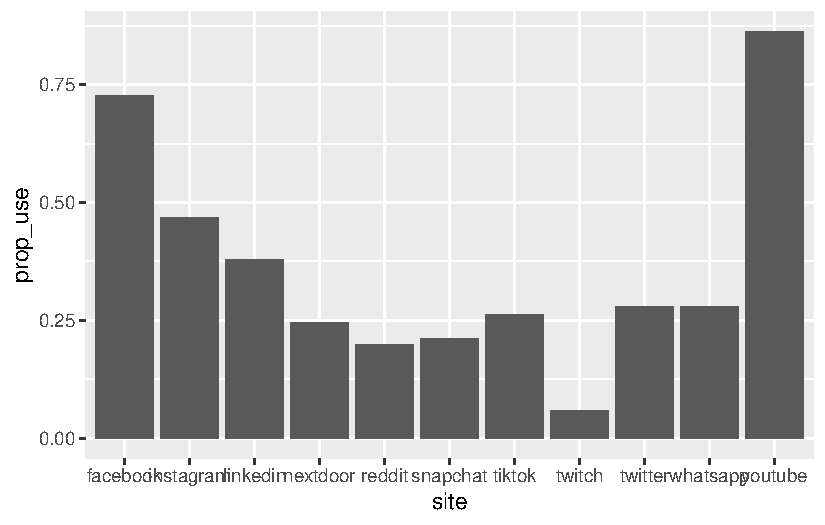
\includegraphics{ps1_ml_files/figure-pdf/unnamed-chunk-21-1.pdf}

}

\end{figure}

That's the basic setup. Now let's use reorder() to order the categories
by value of prop\_use, change the site names to title case, and add
labels to the bars, axes, and plot. You can also shrink and rotate the
axis labels using the theme options.

\begin{Shaded}
\begin{Highlighting}[]
\NormalTok{ps1\_long }\SpecialCharTok{|\textgreater{}} 
  \FunctionTok{group\_by}\NormalTok{(site) }\SpecialCharTok{|\textgreater{}} 
  \FunctionTok{summarise}\NormalTok{(}\AttributeTok{prop\_use =} \FunctionTok{mean}\NormalTok{(use)) }\SpecialCharTok{|\textgreater{}} 
  \FunctionTok{ggplot}\NormalTok{(}\FunctionTok{aes}\NormalTok{(}\AttributeTok{x =} \FunctionTok{reorder}\NormalTok{(}\FunctionTok{str\_to\_title}\NormalTok{(site), prop\_use), }
             \AttributeTok{y =}\NormalTok{ prop\_use)) }\SpecialCharTok{+} 
  \FunctionTok{geom\_col}\NormalTok{() }\SpecialCharTok{+}
  \FunctionTok{geom\_text}\NormalTok{(}\FunctionTok{aes}\NormalTok{(}\AttributeTok{label =} \FunctionTok{round}\NormalTok{(prop\_use,}\DecValTok{3}\NormalTok{), }\AttributeTok{vjust =} \SpecialCharTok{{-}}\NormalTok{.}\DecValTok{25}\NormalTok{), }\AttributeTok{size =} \FloatTok{2.5}\NormalTok{) }\SpecialCharTok{+}
  \FunctionTok{labs}\NormalTok{(}\AttributeTok{x =} \StringTok{""}\NormalTok{, }\CommentTok{\# the values are self explanatory, so leaving title blank is okay}
       \AttributeTok{y =} \StringTok{"Proportion"}\NormalTok{,}
       \AttributeTok{title =} \StringTok{"Social Media Site Usage"}\NormalTok{,}
       \AttributeTok{subtitle =} \StringTok{"Pew Research Center\textquotesingle{}s American Trends Panel (2022)"}\NormalTok{) }\SpecialCharTok{+}
  \FunctionTok{theme}\NormalTok{(}\AttributeTok{axis.text.x =} \FunctionTok{element\_text}\NormalTok{(}\AttributeTok{size =} \DecValTok{9}\NormalTok{, }\AttributeTok{angle =} \DecValTok{45}\NormalTok{, }\AttributeTok{vjust =}\NormalTok{ .}\DecValTok{5}\NormalTok{))}
\end{Highlighting}
\end{Shaded}

\begin{figure}[H]

{\centering 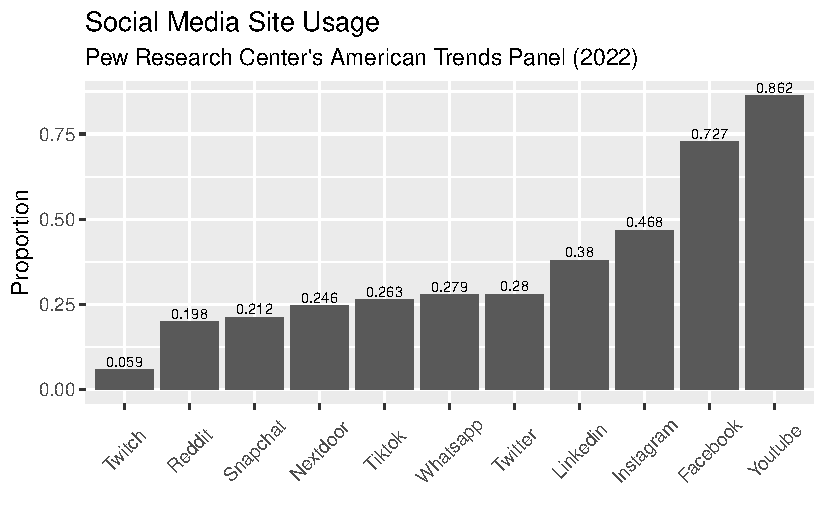
\includegraphics{ps1_ml_files/figure-pdf/unnamed-chunk-22-1.pdf}

}

\end{figure}

The difference for the second plot is that we only want to include users
of the sites. To get them, add a filter before summarizing to get the
mean of the news variable. From the previous figure, we know that we can
filter for use == 1 to restrict our sample to users of each site.

\begin{Shaded}
\begin{Highlighting}[]
\NormalTok{ps1\_long }\SpecialCharTok{|\textgreater{}} 
  \FunctionTok{filter}\NormalTok{(use }\SpecialCharTok{==} \DecValTok{1}\NormalTok{) }\SpecialCharTok{|\textgreater{}} 
  \FunctionTok{group\_by}\NormalTok{(site) }\SpecialCharTok{|\textgreater{}} 
  \FunctionTok{summarise}\NormalTok{(}\AttributeTok{prop\_news =} \FunctionTok{mean}\NormalTok{(news))}
\end{Highlighting}
\end{Shaded}

\begin{verbatim}
# A tibble: 11 x 2
   site      prop_news
   <chr>         <dbl>
 1 facebook     0.410 
 2 instagram    0.264 
 3 linkedin     0.138 
 4 nextdoor     0.220 
 5 reddit       0.322 
 6 snapchat     0.126 
 7 tiktok       0.278 
 8 twitch       0.0948
 9 twitter      0.496 
10 whatsapp     0.115 
11 youtube      0.259 
\end{verbatim}

The code for the figure will be the same setup and another column plot
works well. To add some excitement and show you an alternative, I'll use
geom\_point in the example below and flip the x and y axes (using
coord\_flip) to make the figure more visually appealing.

\begin{Shaded}
\begin{Highlighting}[]
\NormalTok{ps1\_long }\SpecialCharTok{|\textgreater{}} 
  \FunctionTok{filter}\NormalTok{(use }\SpecialCharTok{==} \DecValTok{1}\NormalTok{) }\SpecialCharTok{|\textgreater{}} 
  \FunctionTok{group\_by}\NormalTok{(site) }\SpecialCharTok{|\textgreater{}} 
  \FunctionTok{summarise}\NormalTok{(}\AttributeTok{prop\_news =} \FunctionTok{mean}\NormalTok{(news)) }\SpecialCharTok{|\textgreater{}} 
  \FunctionTok{ggplot}\NormalTok{(}\FunctionTok{aes}\NormalTok{(}\AttributeTok{x =} \FunctionTok{reorder}\NormalTok{(}\FunctionTok{str\_to\_title}\NormalTok{(site), prop\_news), }
             \AttributeTok{y =}\NormalTok{ prop\_news)) }\SpecialCharTok{+} 
  \FunctionTok{geom\_point}\NormalTok{() }\SpecialCharTok{+}
  \FunctionTok{coord\_flip}\NormalTok{() }\SpecialCharTok{+}
  \FunctionTok{geom\_text}\NormalTok{(}\FunctionTok{aes}\NormalTok{(}\AttributeTok{label =} \FunctionTok{round}\NormalTok{(prop\_news,}\DecValTok{2}\NormalTok{), }\AttributeTok{hjust =} \SpecialCharTok{{-}}\NormalTok{.}\DecValTok{25}\NormalTok{), }\AttributeTok{size =} \DecValTok{3}\NormalTok{) }\SpecialCharTok{+}
  \FunctionTok{labs}\NormalTok{(}\AttributeTok{x =} \StringTok{""}\NormalTok{, }\CommentTok{\# the values are self explanatory, so leaving title blank is okay}
       \AttributeTok{y =} \StringTok{"Proportion"}\NormalTok{,}
       \AttributeTok{title =} \StringTok{"Use Of Social Media Site For News"}\NormalTok{,}
       \AttributeTok{subtitle =} \StringTok{"Pew Research Center\textquotesingle{}s American Trends Panel (2022)"}\NormalTok{) }
\end{Highlighting}
\end{Shaded}

\begin{figure}[H]

{\centering 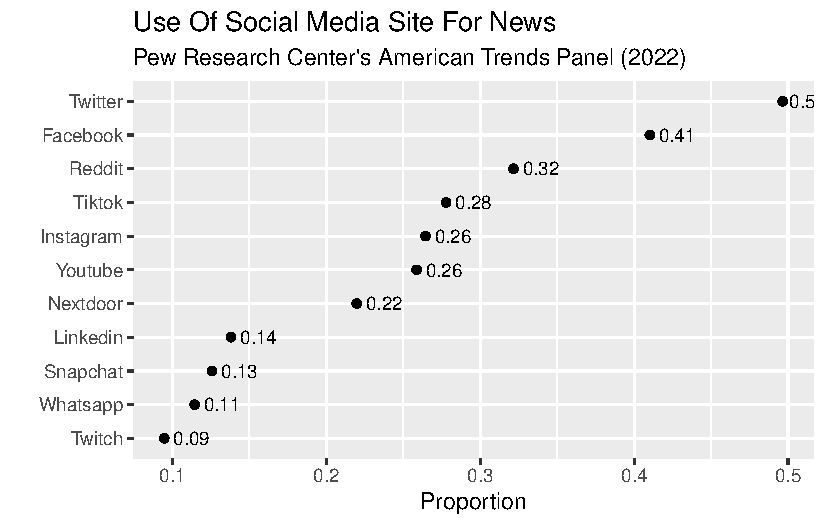
\includegraphics{ps1_ml_files/figure-pdf/unnamed-chunk-24-1.pdf}

}

\end{figure}



\end{document}
